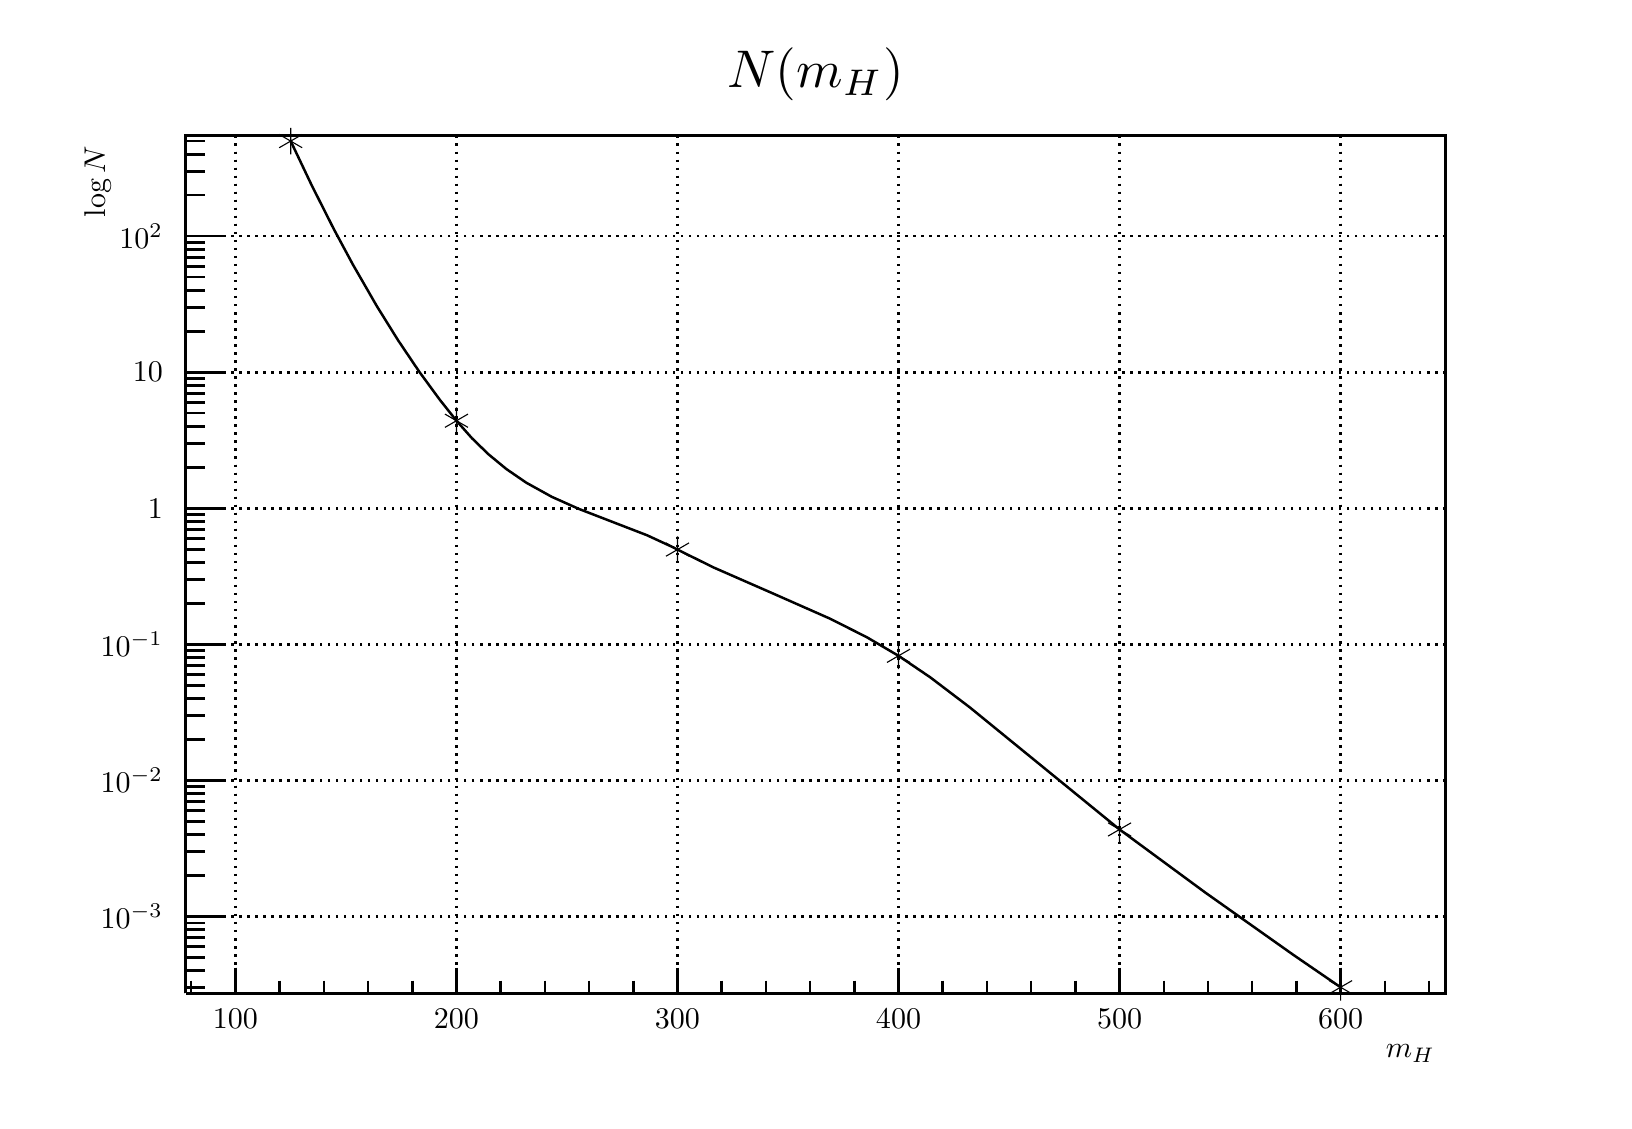
\begin{tikzpicture}
\pgfdeclareplotmark{cross} {
\pgfpathmoveto{\pgfpoint{-0.3\pgfplotmarksize}{\pgfplotmarksize}}
\pgfpathlineto{\pgfpoint{+0.3\pgfplotmarksize}{\pgfplotmarksize}}
\pgfpathlineto{\pgfpoint{+0.3\pgfplotmarksize}{0.3\pgfplotmarksize}}
\pgfpathlineto{\pgfpoint{+1\pgfplotmarksize}{0.3\pgfplotmarksize}}
\pgfpathlineto{\pgfpoint{+1\pgfplotmarksize}{-0.3\pgfplotmarksize}}
\pgfpathlineto{\pgfpoint{+0.3\pgfplotmarksize}{-0.3\pgfplotmarksize}}
\pgfpathlineto{\pgfpoint{+0.3\pgfplotmarksize}{-1.\pgfplotmarksize}}
\pgfpathlineto{\pgfpoint{-0.3\pgfplotmarksize}{-1.\pgfplotmarksize}}
\pgfpathlineto{\pgfpoint{-0.3\pgfplotmarksize}{-0.3\pgfplotmarksize}}
\pgfpathlineto{\pgfpoint{-1.\pgfplotmarksize}{-0.3\pgfplotmarksize}}
\pgfpathlineto{\pgfpoint{-1.\pgfplotmarksize}{0.3\pgfplotmarksize}}
\pgfpathlineto{\pgfpoint{-0.3\pgfplotmarksize}{0.3\pgfplotmarksize}}
\pgfpathclose
\pgfusepathqstroke
}
\pgfdeclareplotmark{cross*} {
\pgfpathmoveto{\pgfpoint{-0.3\pgfplotmarksize}{\pgfplotmarksize}}
\pgfpathlineto{\pgfpoint{+0.3\pgfplotmarksize}{\pgfplotmarksize}}
\pgfpathlineto{\pgfpoint{+0.3\pgfplotmarksize}{0.3\pgfplotmarksize}}
\pgfpathlineto{\pgfpoint{+1\pgfplotmarksize}{0.3\pgfplotmarksize}}
\pgfpathlineto{\pgfpoint{+1\pgfplotmarksize}{-0.3\pgfplotmarksize}}
\pgfpathlineto{\pgfpoint{+0.3\pgfplotmarksize}{-0.3\pgfplotmarksize}}
\pgfpathlineto{\pgfpoint{+0.3\pgfplotmarksize}{-1.\pgfplotmarksize}}
\pgfpathlineto{\pgfpoint{-0.3\pgfplotmarksize}{-1.\pgfplotmarksize}}
\pgfpathlineto{\pgfpoint{-0.3\pgfplotmarksize}{-0.3\pgfplotmarksize}}
\pgfpathlineto{\pgfpoint{-1.\pgfplotmarksize}{-0.3\pgfplotmarksize}}
\pgfpathlineto{\pgfpoint{-1.\pgfplotmarksize}{0.3\pgfplotmarksize}}
\pgfpathlineto{\pgfpoint{-0.3\pgfplotmarksize}{0.3\pgfplotmarksize}}
\pgfpathclose
\pgfusepathqfillstroke
}
\pgfdeclareplotmark{newstar} {
\pgfpathmoveto{\pgfqpoint{0pt}{\pgfplotmarksize}}
\pgfpathlineto{\pgfqpointpolar{44}{0.5\pgfplotmarksize}}
\pgfpathlineto{\pgfqpointpolar{18}{\pgfplotmarksize}}
\pgfpathlineto{\pgfqpointpolar{-20}{0.5\pgfplotmarksize}}
\pgfpathlineto{\pgfqpointpolar{-54}{\pgfplotmarksize}}
\pgfpathlineto{\pgfqpointpolar{-90}{0.5\pgfplotmarksize}}
\pgfpathlineto{\pgfqpointpolar{234}{\pgfplotmarksize}}
\pgfpathlineto{\pgfqpointpolar{198}{0.5\pgfplotmarksize}}
\pgfpathlineto{\pgfqpointpolar{162}{\pgfplotmarksize}}
\pgfpathlineto{\pgfqpointpolar{134}{0.5\pgfplotmarksize}}
\pgfpathclose
\pgfusepathqstroke
}
\pgfdeclareplotmark{newstar*} {
\pgfpathmoveto{\pgfqpoint{0pt}{\pgfplotmarksize}}
\pgfpathlineto{\pgfqpointpolar{44}{0.5\pgfplotmarksize}}
\pgfpathlineto{\pgfqpointpolar{18}{\pgfplotmarksize}}
\pgfpathlineto{\pgfqpointpolar{-20}{0.5\pgfplotmarksize}}
\pgfpathlineto{\pgfqpointpolar{-54}{\pgfplotmarksize}}
\pgfpathlineto{\pgfqpointpolar{-90}{0.5\pgfplotmarksize}}
\pgfpathlineto{\pgfqpointpolar{234}{\pgfplotmarksize}}
\pgfpathlineto{\pgfqpointpolar{198}{0.5\pgfplotmarksize}}
\pgfpathlineto{\pgfqpointpolar{162}{\pgfplotmarksize}}
\pgfpathlineto{\pgfqpointpolar{134}{0.5\pgfplotmarksize}}
\pgfpathclose
\pgfusepathqfillstroke
}
\definecolor{c}{rgb}{1,1,1};
\draw [color=c, fill=c] (0,0) rectangle (20,13.6207);
\draw [color=c, fill=c] (2,1.36207) rectangle (18,12.2586);
\definecolor{c}{rgb}{0,0,0};
\draw [c,line width=0.9] (2,1.36207) -- (2,12.2586) -- (18,12.2586) -- (18,1.36207) -- (2,1.36207);
\definecolor{c}{rgb}{1,1,1};
\draw [color=c, fill=c] (2,1.36207) rectangle (18,12.2586);
\definecolor{c}{rgb}{0,0,0};
\draw [c,line width=0.9] (2,1.36207) -- (2,12.2586) -- (18,12.2586) -- (18,1.36207) -- (2,1.36207);
\draw [c,line width=0.9] (2,1.36207) -- (18,1.36207);
\draw [c,dotted,line width=0.9] (2.63158,12.2586) -- (2.63158,1.36207);
\draw [c,dotted,line width=0.9] (5.4386,12.2586) -- (5.4386,1.36207);
\draw [c,dotted,line width=0.9] (8.24561,12.2586) -- (8.24561,1.36207);
\draw [c,dotted,line width=0.9] (11.0526,12.2586) -- (11.0526,1.36207);
\draw [c,dotted,line width=0.9] (13.8596,12.2586) -- (13.8596,1.36207);
\draw [c,dotted,line width=0.9] (16.6667,12.2586) -- (16.6667,1.36207);
\draw [c,dotted,line width=0.9] (2.63158,12.2586) -- (2.63158,1.36207);
\draw [c,dotted,line width=0.9] (16.6667,12.2586) -- (16.6667,1.36207);
\draw [c,line width=0.9] (2,1.36207) -- (2,12.2586);
\draw [c,dotted,line width=0.9] (18,2.33932) -- (2,2.33932);
\draw [c,dotted,line width=0.9] (18,4.06731) -- (2,4.06731);
\draw [c,dotted,line width=0.9] (18,5.79531) -- (2,5.79531);
\draw [c,dotted,line width=0.9] (18,7.5233) -- (2,7.5233);
\draw [c,dotted,line width=0.9] (18,9.25129) -- (2,9.25129);
\draw [c,dotted,line width=0.9] (18,10.9793) -- (2,10.9793);
\draw [c,line width=0.9] (2,1.36207) -- (18,1.36207);
\draw [anchor= east] (18,0.59931) node[scale=1.08496, color=c, rotate=0]{$m_{H}$};
\draw [c,line width=0.9] (2.63158,1.68897) -- (2.63158,1.36207);
\draw [c,line width=0.9] (3.19298,1.52552) -- (3.19298,1.36207);
\draw [c,line width=0.9] (3.75439,1.52552) -- (3.75439,1.36207);
\draw [c,line width=0.9] (4.31579,1.52552) -- (4.31579,1.36207);
\draw [c,line width=0.9] (4.87719,1.52552) -- (4.87719,1.36207);
\draw [c,line width=0.9] (5.4386,1.68897) -- (5.4386,1.36207);
\draw [c,line width=0.9] (6,1.52552) -- (6,1.36207);
\draw [c,line width=0.9] (6.5614,1.52552) -- (6.5614,1.36207);
\draw [c,line width=0.9] (7.12281,1.52552) -- (7.12281,1.36207);
\draw [c,line width=0.9] (7.68421,1.52552) -- (7.68421,1.36207);
\draw [c,line width=0.9] (8.24561,1.68897) -- (8.24561,1.36207);
\draw [c,line width=0.9] (8.80702,1.52552) -- (8.80702,1.36207);
\draw [c,line width=0.9] (9.36842,1.52552) -- (9.36842,1.36207);
\draw [c,line width=0.9] (9.92982,1.52552) -- (9.92982,1.36207);
\draw [c,line width=0.9] (10.4912,1.52552) -- (10.4912,1.36207);
\draw [c,line width=0.9] (11.0526,1.68897) -- (11.0526,1.36207);
\draw [c,line width=0.9] (11.614,1.52552) -- (11.614,1.36207);
\draw [c,line width=0.9] (12.1754,1.52552) -- (12.1754,1.36207);
\draw [c,line width=0.9] (12.7368,1.52552) -- (12.7368,1.36207);
\draw [c,line width=0.9] (13.2982,1.52552) -- (13.2982,1.36207);
\draw [c,line width=0.9] (13.8596,1.68897) -- (13.8596,1.36207);
\draw [c,line width=0.9] (14.4211,1.52552) -- (14.4211,1.36207);
\draw [c,line width=0.9] (14.9825,1.52552) -- (14.9825,1.36207);
\draw [c,line width=0.9] (15.5439,1.52552) -- (15.5439,1.36207);
\draw [c,line width=0.9] (16.1053,1.52552) -- (16.1053,1.36207);
\draw [c,line width=0.9] (16.6667,1.68897) -- (16.6667,1.36207);
\draw [c,line width=0.9] (2.63158,1.68897) -- (2.63158,1.36207);
\draw [c,line width=0.9] (2.07018,1.52552) -- (2.07018,1.36207);
\draw [c,line width=0.9] (16.6667,1.68897) -- (16.6667,1.36207);
\draw [c,line width=0.9] (17.2281,1.52552) -- (17.2281,1.36207);
\draw [c,line width=0.9] (17.7895,1.52552) -- (17.7895,1.36207);
\draw [anchor=base] (2.63158,0.912586) node[scale=1.08496, color=c, rotate=0]{100};
\draw [anchor=base] (5.4386,0.912586) node[scale=1.08496, color=c, rotate=0]{200};
\draw [anchor=base] (8.24561,0.912586) node[scale=1.08496, color=c, rotate=0]{300};
\draw [anchor=base] (11.0526,0.912586) node[scale=1.08496, color=c, rotate=0]{400};
\draw [anchor=base] (13.8596,0.912586) node[scale=1.08496, color=c, rotate=0]{500};
\draw [anchor=base] (16.6667,0.912586) node[scale=1.08496, color=c, rotate=0]{600};
\draw [c,line width=0.9] (2,1.36207) -- (2,12.2586);
\draw [anchor= east] (0.88,12.2586) node[scale=1.08496, color=c, rotate=90]{$\log N$};
\draw [c,line width=0.9] (2.24,1.43579) -- (2,1.43579);
\draw [c,line width=0.9] (2.24,1.65169) -- (2,1.65169);
\draw [c,line width=0.9] (2.24,1.81915) -- (2,1.81915);
\draw [c,line width=0.9] (2.24,1.95597) -- (2,1.95597);
\draw [c,line width=0.9] (2.24,2.07165) -- (2,2.07165);
\draw [c,line width=0.9] (2.24,2.17186) -- (2,2.17186);
\draw [c,line width=0.9] (2.24,2.26025) -- (2,2.26025);
\draw [c,line width=0.9] (2.48,2.33932) -- (2,2.33932);
\draw [anchor= east] (1.844,2.33932) node[scale=1.08496, color=c, rotate=0]{$10^{-3}$};
\draw [c,line width=0.9] (2.24,2.8595) -- (2,2.8595);
\draw [c,line width=0.9] (2.24,3.16378) -- (2,3.16378);
\draw [c,line width=0.9] (2.24,3.37968) -- (2,3.37968);
\draw [c,line width=0.9] (2.24,3.54714) -- (2,3.54714);
\draw [c,line width=0.9] (2.24,3.68396) -- (2,3.68396);
\draw [c,line width=0.9] (2.24,3.79965) -- (2,3.79965);
\draw [c,line width=0.9] (2.24,3.89986) -- (2,3.89986);
\draw [c,line width=0.9] (2.24,3.98825) -- (2,3.98825);
\draw [c,line width=0.9] (2.48,4.06731) -- (2,4.06731);
\draw [anchor= east] (1.844,4.06731) node[scale=1.08496, color=c, rotate=0]{$10^{-2}$};
\draw [c,line width=0.9] (2.24,4.58749) -- (2,4.58749);
\draw [c,line width=0.9] (2.24,4.89178) -- (2,4.89178);
\draw [c,line width=0.9] (2.24,5.10767) -- (2,5.10767);
\draw [c,line width=0.9] (2.24,5.27513) -- (2,5.27513);
\draw [c,line width=0.9] (2.24,5.41195) -- (2,5.41195);
\draw [c,line width=0.9] (2.24,5.52764) -- (2,5.52764);
\draw [c,line width=0.9] (2.24,5.62785) -- (2,5.62785);
\draw [c,line width=0.9] (2.24,5.71624) -- (2,5.71624);
\draw [c,line width=0.9] (2.48,5.79531) -- (2,5.79531);
\draw [anchor= east] (1.844,5.79531) node[scale=1.08496, color=c, rotate=0]{$10^{-1}$};
\draw [c,line width=0.9] (2.24,6.31548) -- (2,6.31548);
\draw [c,line width=0.9] (2.24,6.61977) -- (2,6.61977);
\draw [c,line width=0.9] (2.24,6.83566) -- (2,6.83566);
\draw [c,line width=0.9] (2.24,7.00312) -- (2,7.00312);
\draw [c,line width=0.9] (2.24,7.13994) -- (2,7.13994);
\draw [c,line width=0.9] (2.24,7.25563) -- (2,7.25563);
\draw [c,line width=0.9] (2.24,7.35584) -- (2,7.35584);
\draw [c,line width=0.9] (2.24,7.44423) -- (2,7.44423);
\draw [c,line width=0.9] (2.48,7.5233) -- (2,7.5233);
\draw [anchor= east] (1.844,7.5233) node[scale=1.08496, color=c, rotate=0]{1};
\draw [c,line width=0.9] (2.24,8.04347) -- (2,8.04347);
\draw [c,line width=0.9] (2.24,8.34776) -- (2,8.34776);
\draw [c,line width=0.9] (2.24,8.56365) -- (2,8.56365);
\draw [c,line width=0.9] (2.24,8.73111) -- (2,8.73111);
\draw [c,line width=0.9] (2.24,8.86794) -- (2,8.86794);
\draw [c,line width=0.9] (2.24,8.98362) -- (2,8.98362);
\draw [c,line width=0.9] (2.24,9.08383) -- (2,9.08383);
\draw [c,line width=0.9] (2.24,9.17222) -- (2,9.17222);
\draw [c,line width=0.9] (2.48,9.25129) -- (2,9.25129);
\draw [anchor= east] (1.844,9.25129) node[scale=1.08496, color=c, rotate=0]{10};
\draw [c,line width=0.9] (2.24,9.77147) -- (2,9.77147);
\draw [c,line width=0.9] (2.24,10.0758) -- (2,10.0758);
\draw [c,line width=0.9] (2.24,10.2916) -- (2,10.2916);
\draw [c,line width=0.9] (2.24,10.4591) -- (2,10.4591);
\draw [c,line width=0.9] (2.24,10.5959) -- (2,10.5959);
\draw [c,line width=0.9] (2.24,10.7116) -- (2,10.7116);
\draw [c,line width=0.9] (2.24,10.8118) -- (2,10.8118);
\draw [c,line width=0.9] (2.24,10.9002) -- (2,10.9002);
\draw [c,line width=0.9] (2.48,10.9793) -- (2,10.9793);
\draw [anchor= east] (1.844,10.9793) node[scale=1.08496, color=c, rotate=0]{$10^{2}$};
\draw [c,line width=0.9] (2.24,11.4995) -- (2,11.4995);
\draw [c,line width=0.9] (2.24,11.8037) -- (2,11.8037);
\draw [c,line width=0.9] (2.24,12.0196) -- (2,12.0196);
\draw [c,line width=0.9] (2.24,12.1871) -- (2,12.1871);
\draw [c,line width=0.9] (3.33333,12.1871) -- (3.601,11.6238) -- (3.88212,11.0675) -- (4.12155,10.622) -- (4.42858,10.0889) -- (4.69734,9.65726) -- (4.96587,9.25859) -- (5.22604,8.90334) -- (5.4386,8.63573) -- (5.63396,8.41501) -- (5.84312,8.21138)
 -- (6.07222,8.0224) -- (6.3262,7.84823) -- (6.65216,7.66792) -- (6.99532,7.51503) -- (7.85983,7.18091) -- (8.1942,7.02622) -- (8.24561,6.99936) -- (8.70165,6.77329) -- (9.46186,6.44037) -- (10.1841,6.12139) -- (10.6506,5.886) -- (11.0526,5.65035) --
 (11.4546,5.37779) -- (11.9587,4.99483) -- (13.8596,3.44487) -- (14.9479,2.64413) -- (16.0634,1.85476) -- (16.6667,1.44114);
\foreach \P in {(3.33333,12.1871),(5.4386,8.63573),(8.24561,6.99936),(11.0526,5.65035),(13.8596,3.44487),(16.6667,1.44114)}{\draw[mark options={color=c,fill=c},mark size=4.804805pt,mark=asterisk] plot coordinates {\P};}
\draw (10,13.0353) node[scale=1.91463, color=c, rotate=0]{$N(m_{H})$};
\end{tikzpicture}
